\section{Conclusions}
\label{sect:conclusions}

%Summarize conclusions and say how this thesis has expanded knowledge in the area of interest.

%Critical assessment of own work. State hypothesis, and demonstrate precision, thoroughness, contribution, and comparison with closest rival.

\subsection{Metrics}
 In Sect.~\ref{sect:metrics} a number of Complexity (C) and Quality (Q) metrics were considered. Demand $C_D$ and contention $C_C$ were suggested as useful measures of the complexity of a scheduling problem. Later in Sect~\ref{}  it was shown that contention can also provide an indication of the potential utility achievable by a scheduler, in that complex (high $C_C$ and $C_D$) ODBs tend to give higher overall quality measures. Basically there are likely to be a higher population of quality observations to choose from and so more chance these will be selected than in a low contention ODB, where at times low quality observations might be chosen for lack of anything better.

 A general utility measure combining user and enterprise measures of quality was suggested (Eq.~\ref{eq:utility}) and provides a potentially interesting area for further study. 

For the current thesis a set of simpler (primitive) quality measures were designed and used in the simulation experiments. Some associations were suggested between these quality metrics and the accepted scheduling and planning timescales. Of the available utility measures, the two most promising for future use in longer term planning are the yield tracking ($Q_{YT}$) and target demand ($Q_{TD}$) metrics. They are also the most challenging and time-consuming to calculate and for this reason were not used seriously other than in the early shakedown experiments as proof of concept. 

\subsection{Characterization of operating environment}
 A detailed study of the operating environment was made, gathering information from a variety of sources with a view to employing this information in developing future longer horizon scheduling and planning systems. 

%\subsubsection{Weather}
 Meteorological information was obtained from logs of the telescope's own weather monitoring system (WMS) and from nightly observing logs. In terms of the telescope, weather is classed as good or bad depending on whether a specific set of conditions are satisfied. The weather on site was found to be good for about 80\% of the time averaged over the year. There is, perhaps not surprisingly, generally more good weather in summer than winter. Typically it was found that there is $<5$\% bad weather in June rising to as much as 60\% in February.

 The major contribution to bad weather is high humidity accounting for around 18\% of such time. Other factors such as high winds and freezing temperatures account for only a few percent of the bad weather. 

Using an analysis of the distribution of lengths of good and bad periods, a simple prediction model was designed in which it was assumed the weather would continue in its current condition for a period similar in length to the amount of time which it has already been in that state but with an exponentially decaying likelyhood of changing to the alternate state. This model was tested against recorded data and was found capable of anticipating the length of the current period of weather with a degree of accuracy exceeding the long-term average for upto 30 hours ahead though with decreasing accuracy. 
Further analysis of the WMS data shows that continuous runs of bad weather (days on which the amount of time classified as bad exceeds a specified threshold) indicate that for a threshold of ??? 90\%, around 50\% of bad weather runs are $<5$ days long with $<10$\% of runs exceeding 15 days. This information could be useful in longer-horizon planning, for instance to determine whether a particular group might be observable in the next few nights or whether it would be safer to observe it tonight.

%\subsubsection{Seeing}
Details of the atmospheric seeing, measured by a real-time pipeline operating on data from the telescope's main imaging camera (RATCAM), were extracted from the data archive and reduced taking into account pixel-scale, binning, filter wavelength and target elevation above the horizon. The results indicated that the median seeing on site is around 0.95''. It was also noted that median seeing is best in summer, typically around 0.78'' with average of 1.0'' and poorest in December with a median value around 0.93'' and average over the winter months of 1.5''. It was further found that typically, and contrary to popular belief, no measurable variation in seeing quality occurs over the course of the night.


 %\subsubsection{Extinction}


 %\subsubsection{downtime}
Using technical downtime information from the nightly operations logs gathered over a period of the first 3 years of operation of the telescope it was found that most nights ($>72$\%) have less than 5\% downtime while some 8\% of nights suffered nearly 100\% downtime. In terms of use in prediction, there was no readily discernable pattern to technical downtime.
 
% \subsubsection{phase2 content}


\subsection{Architecture}
The original brief was to develop an architecture with which to build a variety of schedulers along with a simulation framework with which to characterize and test schedulers on a variety of scheduling scenarios. Initial work on the LT scheduler deployed at the start of robotic operations provided clues as to the range of components which would be required. 

A comprehensive architecture was then designed taking into account these considerations. The architecture contains a large number of pluggable interface components which allow numerous scheduling paradigms to be created. In the subsequent experiments two main paradigms were tested. BDS is a simple despatch scheduler while QLAS is a look-ahead scheduler with a pre-designated horizon size. 

Using the simulation framework, the pluggable nature of the architecture allowed a number of experimental contollers to be quite straightforwardly setup and used to test the schedulers. The number of components available means that for anyone else using the framework there would be something of a learning curve required to use it, however much of the setup is fairly standard and it has proved easy to simply use an existing simulation controller as a template, then by making small changes to just one or two models adapt it to perform alternative experiments. Often just the Phase 2 model needs changing to create a different population distribution or to vary the seeding of high-valued groups.

Much of the information gained in developing the framework leads me to feel that it would be quite feasible to extend the use of this architecture to other projects, perhaps with radically different Phase 2 concepts despite the critical dependance of much of the architecture on the very nature of the adopted Phase 2 model. In such a case it would be neccessary for either the project to adapt its Phase 2 concept to match the one used in this thesis or to adapt the architecture to an alternative Phase 2 model. 

\subsection{Experiments}

\begin{description}
\item[Man against Machine]
It was shown that a human scheduler using rules which may not be known to the scheduler himself is capable of generating effective, high-quality schedules as measured by the various Q metrics. In some cases the human scheduler was able to outperform an automated (BDS) scheduler on certain metrics. By studying the variation of quality metrics against those of the automated scheduler it was possible to deduce the approximate relative weighting factors used by the human scheduler as being given approximately by $0.8 f_{el} + 0.2 f_{pr}+ \epsilon f_{rn}$ where $\epsilon$ is very small ($\ll 0.1$).

 \item[Scoring]
 This series of investigation showed that the effect of changing the weights applied to the various heuristic metrics used in making scheduling decisions have little effect on each other. When we change any given f metric the corresponding Q metric is affected though not as much as might have been anticipated. There is generally little effect on any other Q metric. The choice of weighting determines the character of the schedule but only the dominant f metric has any real effect while the other metrics appears like noise and suppress the effectiveness of the chosen f metric. The overall conclusion that can be taken from this is that whatever qualities we want from a schedule must be actively selected for in the scoring and selection models. 
 \item[Complexity]
 In order to compare the capabilities of generated Phase 2 models with those from real ODB snapshots a series of experiments was performed. These experiments also investigated the effect of database (Phase 2) complexity or \emph{weight}, measured using the average contention measure $C_C$ on scheduling. It was found that by suitable adjustment of the generator parameters, models could be created with similar characteristics to real ODB snapshots. There was however significant variation in the qualities of these models. The scheduling experiments showed that at low levels of complexity there is considerable variation in the fullness ($Q_{XT}$) of schedules generated by all scheduling paradigms. As the level of complexity increases the degree of variation decreases. The variation in quality ($Q_{SU}$) was found to be fairly constant at all levels of complexity but the average value was seen to increases with complexity for all scheduling paradigms whether despatch or look-ahead. It was also found that as the look-ahead horizon increases there is a general (though small) increase in quality with complexity. 

 \item[Stability]
Using a QLAS scheduler it was found that as the degree of environmental stability increased we could profit significantly by employing longer look-ahead horizons. The rate of increase in the amount of improvement is seen to diminish with longer horizon lengths. It was also found that by increasing the number of trials (a QLAS search control parameter) we could also achieve improvements, again however, the rate of increase was slow. This is a natural consequence of the random search mechanism employed, we should expect to see much faster improvements with a proper heuristic search mechanism in place. It was found that BDS could outperform any of the QLAS implementations when the environmental stability time $\tau_E$ was less than the look-ahead horizon, but that once $\tau_E \apprge H$ the LAS performance exceeds that of BDS. 

 \item[Volatility]
Embedded instrumentation was used to record changes to the Phase 2 ODB, termed volatile events. Some simple metrics were designed with which to characterize these events. It was found that at busy times upto 50\% of the nights potential observations can arrive after the start of night's observing.

In simulation experiments it was found that for any given look-ahead horizon H there was an optimum value of proximity (one of the characterization metrics) at which the highest relative improvement occured. This was found to be related to H (details). An enhanced look-ahead scheduler, ELAS which included a sequestration policy was introduced and this was seen to yield further improvement in schedule quality. The effectivenss of ELAS relative to QLAS was seen to increase with increasing horizon length.

\item[Disruption]
Disruptive events, breaks in the natural execution cycle due to weather, mechanical or computer problems were investigated to determine their effect on schedule quality. It was found that for a given total disruption time, a large number of small disruption had a worse effect than a few long events. The effect was seen to be more pronounced for longer look-ahead horizons. The despatch schedulers were unnaffected, the \emph{myopic advantage}.

 \item[Prediction accuracy]
The effects resulting from the accuracy with which we are able to predict the environmental stability timescale was investigated. It was found that when determining the horizon length, if we either over or under-estimate the duration of stable conditions we get poorer results. The optimum situation appears to be when $H \simeq f\tau_E$ where $f$ is around 0.7 to 0.8.
\end{description}

\subsection{Summary}
% aim
A principle aim of this thesis was to develop the tools with which to build an adaptive scheduler and to determine under what conditions such adaptive behaviour would be neccessary. We have established that the two scheduling paradigms investigated do indeed behave differently with respect to operating conditions and that in particular the \emph{stability} or \emph{smoothness} of the operating environment is a critical factor in determining both which type of scheduler to employ and how it should be configured.

% bds versus las and stability
 BDS is a \emph{myopic} scheduler, it can only see what it is doing at the time and knows nothing about what future decisions it might need to make. This can be both an advantage and disadvantage. Under rapidly changing conditions, this myopism is a definite advantage. A look-ahead scheduler which is committed to its decisions for a period may suffer because either the conditions improve and it has already chosen to perform low quality observations, or the conditions deteriorate and the previously committed high quality observations become non-viable. The effects of large numbers of disruptions and volatile events have a similar effect in that future commitments may have to be broken to accomodate these effects, thus reducing the look-ahead advantage. BDS on the other hand does not see any of this instability and is able to respond instantly to changes.

Under stable conditions, we have seen that provided we are able to estimate the degree of stability accurately, the choice of a long look-ahead horizon gives considerably better results than simple despatching.

% design
A design for the adaptive scheduler is now suggested. It is clear that we need a way of accurately predicting these variables ahead for at least the length of the longest horizon we might consider. Once we have this information we can choose a look-ahead horizon to be roughly the length of the shortest stability period. However, when conditions are very \emph{rough} in any of the operating parameters we should revert to despatch scheduling. The work of Sect.~\ref{sect:volanal} also informs us that both an effective break policy and sequestration policy will help us to mitigate against instability so a scheduler like ELAS is more useful than QLAS.

The look-ahead schedulers tested used a very inefficient search algorithm. Though perfectly accceptable for simulation experiments where time was not an issue, this would need to be improved upon significantly for an operational system.

% combined utility
It is clear from Sect.~\ref{sect:metrics} that there is no \emph{magic} quality metric which can be used to determine the optimum schedule. The decision on which metrics to use are very much dependant on operational and management preferences. The combined utility metric (Eq.~\ref{eq:utility}) discussed in Sect.~\ref{sect:sqms} incorporating both enterprise and user preferences is suggested as the way ahead.

% forward planning over operational and tactical timescale
It seems reasonable to suggest that a degree of forward planning might be useful. I have already alluded (Sect.~\ref{sect:matchmetrics}) to the yield-tracking and urgency metrics ($Q_{YT}$ and $Q_{RN}$) and how these might be useful in this context. Fig.~\ref{fig:plan_sched} shows a possible way in which longer-term planning could be integrated. The higher planning layers use long-term quality metrics (fed through statistics from lower levels) to assess whether the scoring metrics and weights at those lower levels should be varied.

 The work in Sect.~\ref{ss:conc_pred} on forward prediction of weather condtions and run-length distributions could be useful in this context. An example might be where a group of high quality might be observed on several of the next few nights. However, it would be better to observe in 2 nights time if possible - perhaps the moon will be further from the target or the seeing is not especially good tonight. In such a case we would need to balance the likelihood of conditions improving over the next few nights against the possibility of the weather deteriorating to the extent that the group cannot actually be observed on those nights. Such effects could for example be taken into account using a scoring mechanism including a discounted future reward term (Eq.~\ref{eq:discountreward}). 

   \begin{figure}[htp]
   \begin{center}
   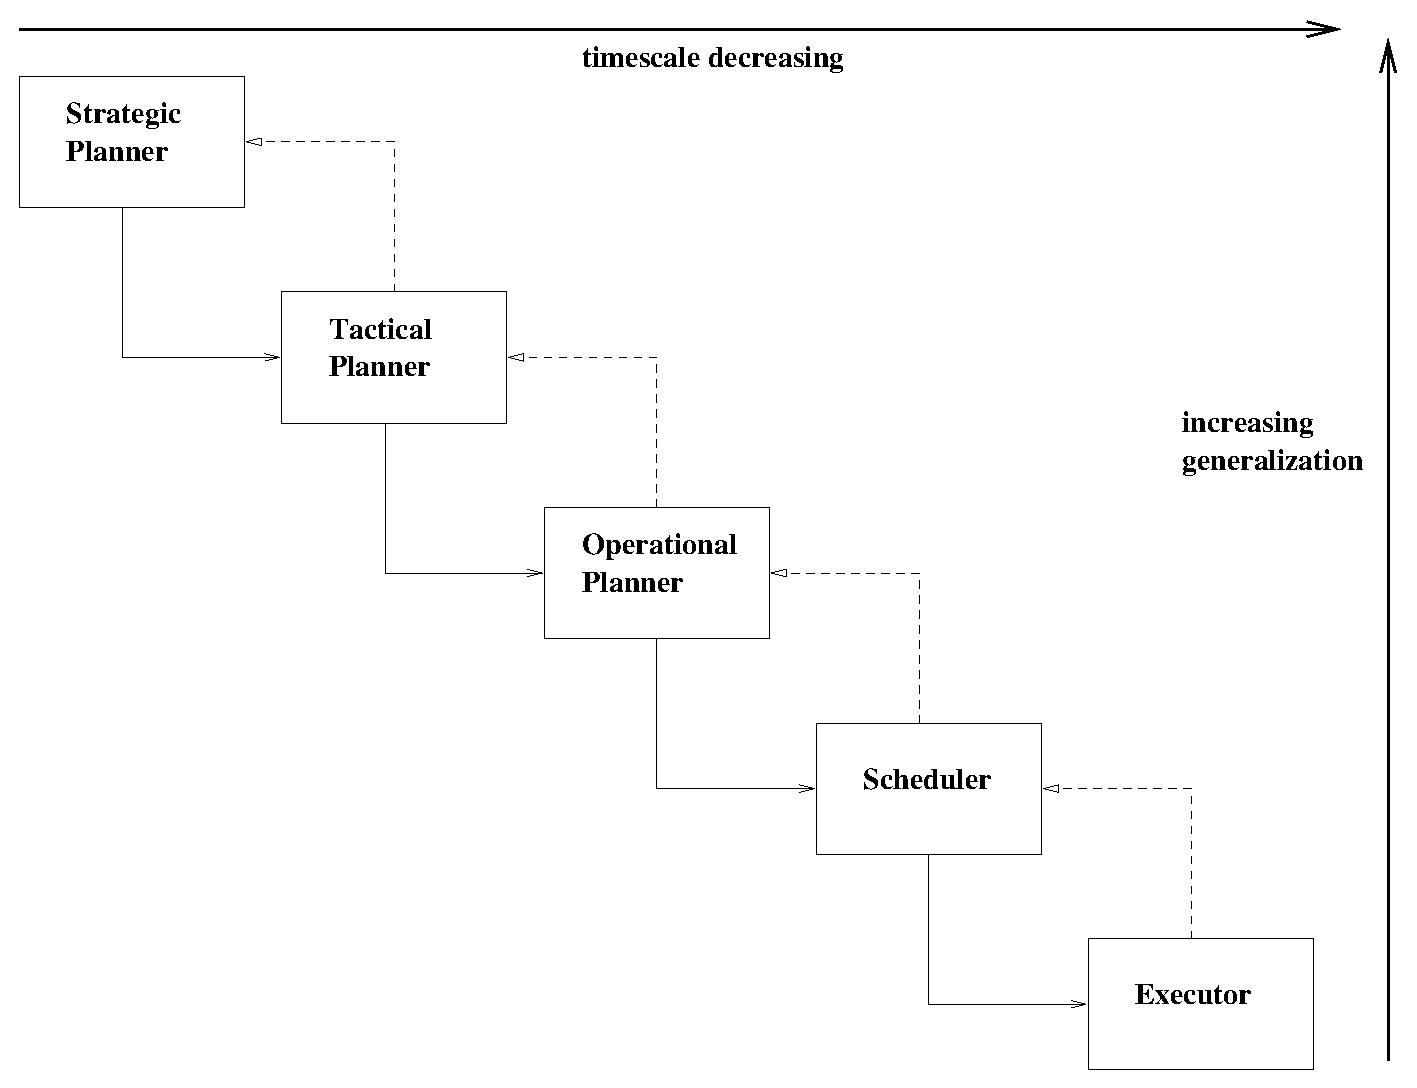
\includegraphics[height=6cm]{figures/plan_sched.eps}
   \end{center}
   \caption[Interaction between planning and scheduling.] 
   {Interaction between planning and scheduling...expand}
   \label{fig:plan_sched} 
   \end{figure} 

\section{Further work}
\label{sect:further}

With reference to Fig.~\ref{fig:las_feedback} which shows how the adaptive elements could integrate into the scheduler, there are a number of things which need implementing before an Adaptive Look-Ahead Scheduler (ALAS) can be used for operational scheduling. Several of the specialized modules must be designed and written and the search mechanism must be speeded up.


   \begin{figure}[htp]
   \begin{center}
   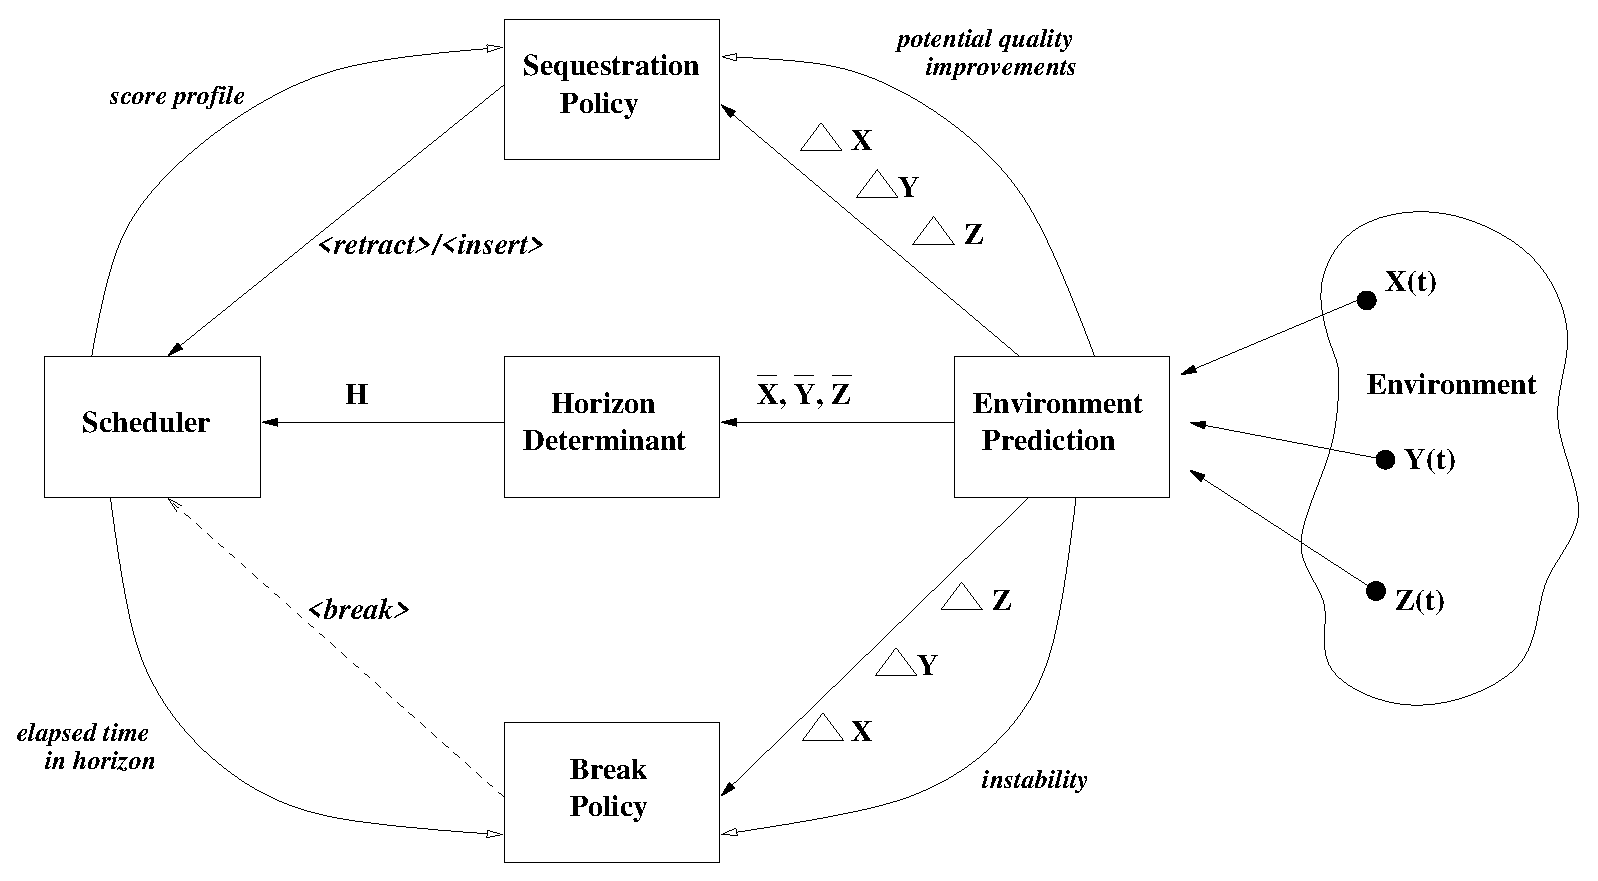
\includegraphics[height=6cm]{figures/las_feedback.eps}
   \end{center}
 
   \caption[Environmental prediction in scheduling architecture.] 
   {Simplified architecture to allow environmental prediction to influence the scheduler. The \emph{HorizonDeterminant} uses details of stability to decide on the current horizon. Volatile events (typically a surge of new observations) are fed to the \emph{SequestrationPolicy} to decide whether to modify the running schedule by retracting existing commitments and inserting new ones. Changes to environmental stability are fed to the \emph{BreakPolicy} to determine whether to stop the current schedule and reschedule or to carry on with reduced value.}
   \label{fig:las_feedback} 
   \end{figure} 


 Although we have looked at how stability and other environmental conditions affect the scheduling process, we have assumed we can actually determine this information. Infact such prediction is not easy.

\begin{description}
\item [External forecasting sources]
We already have access to and use internal weather and sky monitoring systems. Ideally however, we should be able to obtain information from various external sources:- short and medium range weather forecasts are available from the European Centre for Medium Range Weather Forecasting (ECMWF). Atmospheric seeing and extinction forecasts are available from MeteoBlue. \cite{marchant09forecast} has performed an analysis on the accuracy of MeteoBlue predictions of weather parameters for several days ahead and found around 70\% agreement over that timescale. 

\item [Sensor fusion]
There is potential for a significant amount of work on fusing these sources information together to make stability predictions. The forecast information exists on different timescales which might point to different sources being applicable to the different planning timescales. We should not ignore the option to use human input. Humans are good at extracting predictive information from very complex datasets - it could prove most effective to have an interactive input to the scheduler where an interpreter sets out the probabilities of bad weather based on detailed study of a variety of forecast sources. 

\item [Texture based metrics]
Could look at texture measurement for prediction of complexity.

\end{description}

Both QLAS and ELAS are very inefficient due to the random solution generation/search process. This is not par ticularly important in a simulation context - other than in the time taken to perform the simulations. However, in an operational context where solutions need to be found quickly to avoid holding up the execution, more  efficient and intelligent solution generation and search mechanisms would be required.

\begin{description}

 \item [Solution generator and search mechanism]
There are several heuristic techniques which might be used to speed up the generation of solutions to test.

\begin{itemize}
\item \emph{Breeder} Genetic techniques might be used to breed solutions. In any potential sequence solution there will be good (high scoring) segments and poorer (low scoring) segments. In some cases the good part might be early in the sequence while in another it might be nearer the end. If we were to take the good parts of one solution and merge these with the good parts of another solution we could create a new solution with more good parts then either parent. Similarly, we might find that by changing just a few components in an already good solution we could achieve a better solution. These two techniques represent in effect the genetic mechanisms of \emph{crossover} and \emph{mutation}. There are potential options to speed this mechanism up by farming out the breeding to a number of seperate \emph{breeder stations} running in parallel on different hosts.

\item \emph{Energy minimization} This technique assumes that each group excerts a repulsive force on all surrounding groups which might be in competition for the same region of the time axis. The force excerted would be related to the importance and urgency of the group (its score). \emph{Strong} groups would be able to claim their ideal location on the timeline whereas \emph{weak} groups woould be forced off into less desirable regions (from their point of view) or even ejected if a strong group required the whole of the weak group's feasible window.

\end{itemize}

 \item [Break policy]
Notifications of instability need to be integrated into the system so that decisions can be made as to when to curtail the execution of the current sequence and recalculate.

 \item [Sequestration policy]
To take advantage of improvements in the conditions or the arrival of better quality observations, a sequestration policy must be devised to allow the executing schedule to be re-calculated or modified.

 \item [Retraction heuristics]
When responding to a sequestration, the retraction heuristic determines the choice of group to replace.


 \item [Expected Future Reward]
I have already briefly discussed the possibility of using Expected Future Reward (EFR) in the context of determining whether to schedule a group now or at some later point based on the likelyhood of suitable conditions. This technique allows one to \emph{hedge one's bets} against future uncertainty by discounting the return from decisions made in the present. A study by \cite{sozou98hyperbolic} reveals that humans typically use a form of discounting where the perceived hazard rate changes with time yielding a hyperbolic discount rate. They provide mechanisms whereby a discount rate can be calculated based on non-occurance of a perceived risk using Bayesian updating and also note that such non-exponential time-preference curves can cross-over so that preferences may change. The main research interest in this area would be in the determination of a suitable discount rate with reference to predicted and observed stability and volatility measures.

\end{description}


There are some areas in which the Phase 2 model could be enhanced to provide additional features...why?

\begin{itemize}

 \item User preferences. So far, the scoring mechanism has been biased toward enterprise measures of reward (Sect.~\ref{sect:sqms}) and little regard has been taken of the individual user's measures of value. It is true that for instance the relative elevation of targets is taken into account to ensure that targets are observed at \emph{good} times, however we do not allow the trade-offs between the various user-preferences to be made. The Phase 2 model could be enhanced to allow it to represent user's own quantification of these tradeoffs.


 \item Quality requirements. There might be some merit in allowing users to specificy limits on the amount, regularity and quality of data taken. Currently when a group fails for whatever reason it becomes reschedulable and no charge is made. In some cases, most of the required observations might have been made anyway. In such situations it would increase effciency if a QOS measure could be used to determine the degree of success rather than the present hard cutoff rule.

% \item Auctions for preference matching.

\end{itemize}

